The SaltNet architecture is designed with a multi-pathway approach to effectively denoise images while maintaining computational efficiency. As depicted in Figure \ref{fig:saltnet_architecture}, the network ingests a grayscale noisy image and processes it through several parallel pathways before converging to produce the final denoised output. This structure allows SaltNet to leverage different denoising strategies, addressing various noise types effectively.

\begin{figure}[h]
    \centering
    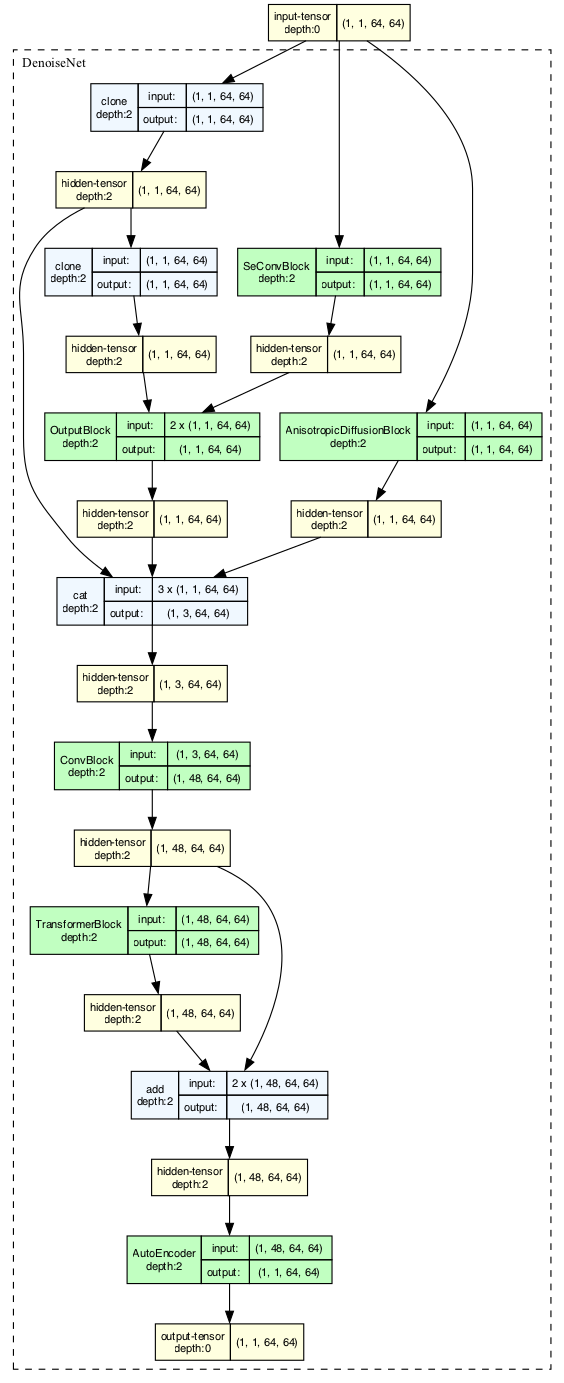
\includegraphics[width=0.8\textwidth]{assets/network_architecture.png}
    \caption{SaltNet Architecture Diagram}
    \label{fig:saltnet_architecture}
\end{figure}

The input noisy image, represented as a tensor of dimensions \( (1, 1, InputHeight, InputWidth) \), is initially cloned and fed into two distinct branches: a stack of Selective Convolutional (SeConv) blocks and a stack of novel Anisotropic Diffusion blocks.

The first branch utilizes \textbf{SeConv blocks}, inspired by the SeConvNet architecture\cite{Rafiee2021}, to effectively address salt-and-pepper noise. We employ a stack of \texttt{7} SeConv blocks, each with increasing kernel sizes to capture multi-scale features. The output of the SeConv block stack is passed through a single \texttt{OutputBlock}: a Conv2d layer, batch normalization layer and ReLU activation, as opposed to a deep CNN network  in the original SeConvNet architecture.

Concurrently, the input image is also processed by a novel stack of \textbf{Anisotropic Diffusion blocks}. This branch uses a novel block implementation, drawing inspiration from anisotropic diffusion filtering but implemented within a deep learning framework. We stack \texttt{5} of these blocks, each applying a learned anisotropic diffusion process to smooth noise while preserving edges and image structures. This component is particularly effective in handling probalistic noise types, such as Gaussian and Poisson noise.

The outputs from both the SeConv and Anisotropic Diffusion branches, along with a cloned version of the original noisy input, are then concatenated along the channel dimension. This concatenated tensor, now with \texttt{3} input channels, is passed into a \textbf{Convolutional Embedding Layer} (\texttt{ConvBlock}). This layer, consisting of a convolutional layer, batch normalization, and ReLU activation, serves to create a feature embedding space with \texttt{48} channels, effectively fusing information from the different denoising pathways.

The resulting feature embeddings are then processed by a small number of \textbf{Transformer blocks}, specifically \texttt{10} blocks. Inspired by the Restormer architecture\cite{Zamir2022}, these transformer blocks leverage multi-head attention mechanisms to capture long-range dependencies within the image. This allows the network to model global image context. To maintain computational efficiency, we limit the number of transformer blocks, compared to deeper Restormer architecture.

Finally, the output of the transformer blocks is fed into an \textbf{AutoEncoder} module. This module inspired by U-Net with skip connections\cite{Wu2022} acts as a post-processing refinement stage. The AutoEncoder, with a depth of \texttt{5}, further refines the denoised features and projects them back to the single-channel grayscale image space. It takes in an input of 48 channel dimensions and produces the final denoised output tensor of dimensions \( (1, 1, InputHeight, InputWidth) \).

By combining these components, SaltNet achieves a robust and efficient denoising architecture. The parallel processing branches allow for specialized handling of different noise characteristics, while the Transformer blocks and AutoEncoder ensure high quality in the final denoised images. This multi-pathway approach, positions SaltNet as a competitive and efficient alternative to existing state-of-the-art denoising networks like Restormer.
